
\chapter{Arquitetura de Software}
\label{sec-arquitetura}
\vspace{-1cm}

A Figura~\ref{figura-arquitetura} mostra a arquitetura do sistema \emph{\imprimirtitulo}.

\begin{figure}[h]
	\centering
	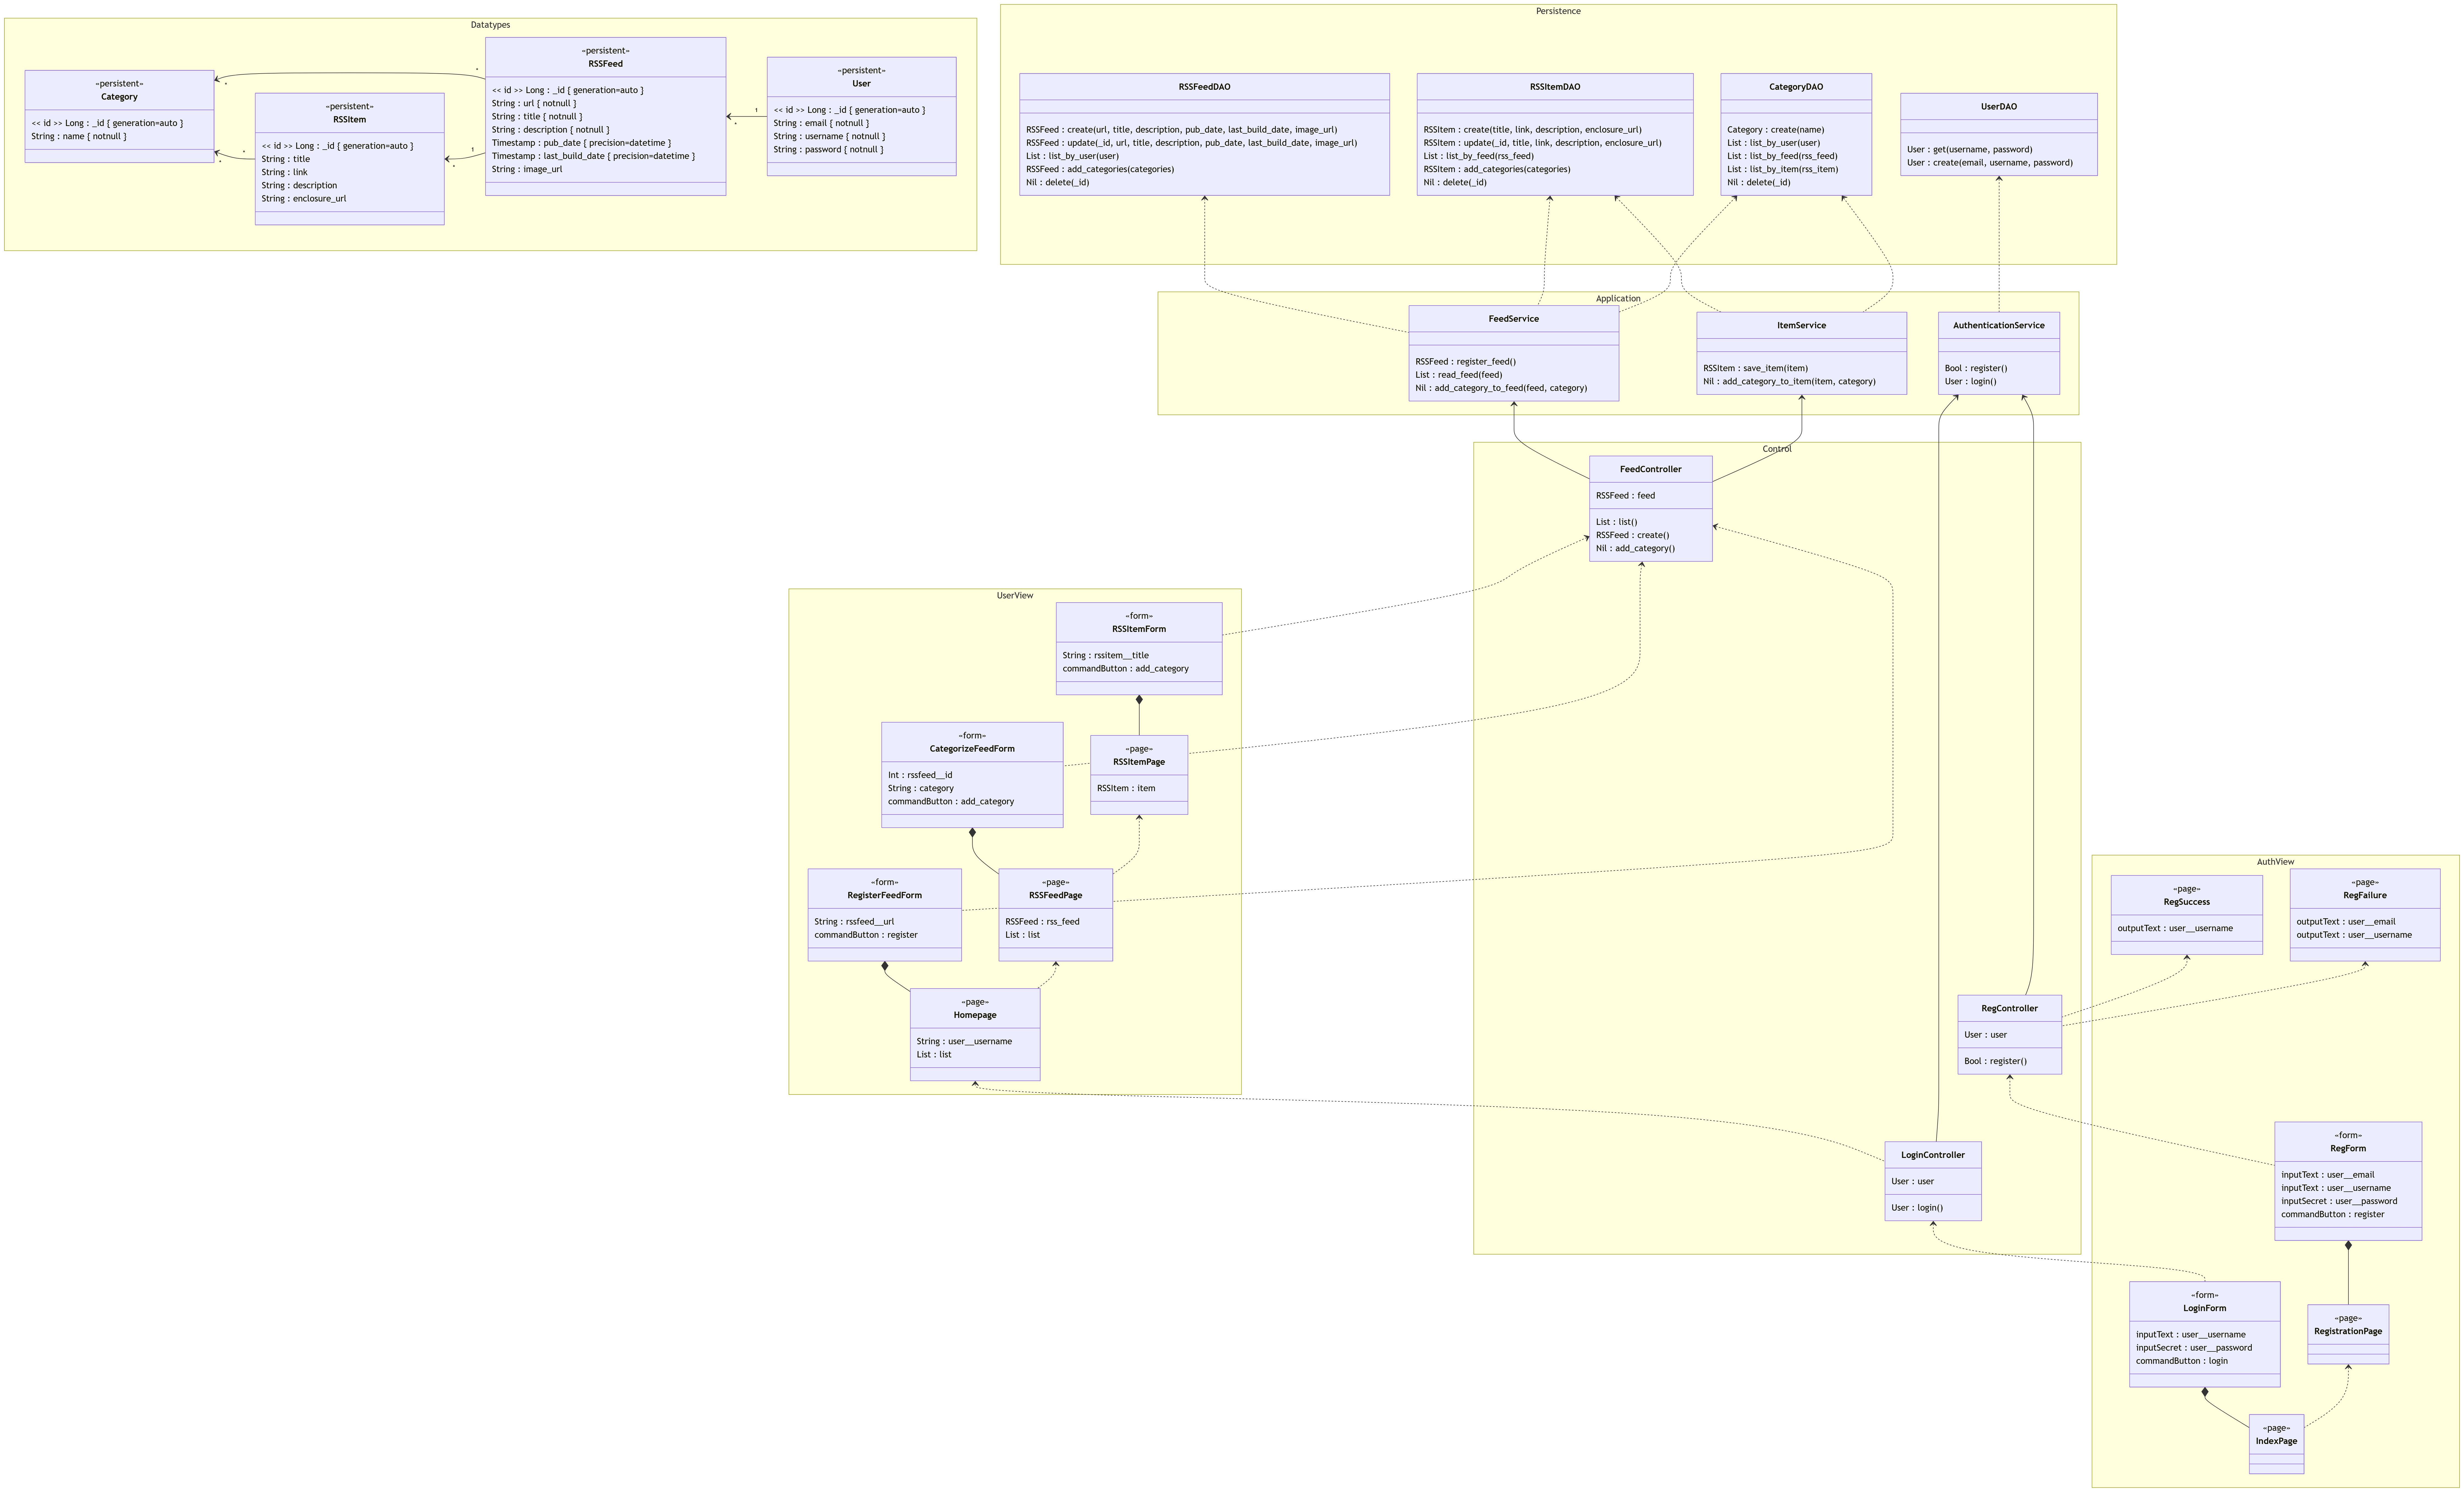
\includegraphics[width=0.8\textwidth]{figuras/Modelo-FrameWeb}
	\caption{Arquitetura do sistema.}
	\label{figura-arquitetura}
\end{figure}

%\vitor{Substituir a Figura~\ref{figura-arquitetura} pelo diagrama UML da arquitetura do seu projeto e descrevê-la no texto. Caso use alguma arquitetura clássica, incluir referência bibliográfica com BibTeX (ex.:Camada de Serviço~\cite{fowler:book02}). Como exemplo, vide documento de projeto do Marvin.}

Podemos ver que a aplicação é divida em seis pacotes: um para a definição dos tipos do domínio, um para persistência de dados, dois para controlar a navegação visual da aplicação, e dois para realizar a comunicação entre a navegação e a persistência.

A ideia é que os pacotes \textit{Application} e \textit{Persistance} farão parte do \textit{back-end}, enquanto que os pacotes \textit{Control}, \textit{UserView} e \textit{AuthView} farão parte do \textit{front-end}. O pacote \textit{Datatypes} será referenciado pelas duas pontas da aplicação, já que representa a estrutura que os dados terão durante a execução da lógica do domínio.

A ideia é que um usuário pode realizar o cadastro na aplicação, o que o permite que ele possa salvar links de feeds RSS na sua conta, e também possa editar as categorias às quais tanto os feeds quanto os itens dos feeds pertencem, por isso estamos salvando esses dados no banco. Isso também permite que, numa suposta versão futura da aplicação, seja possível mostrar o conteúdo de um item do feed dentro de sua página.